\documentclass[a4paper]{article}  

\usepackage{mathtools}
\usepackage{amsthm}
\usepackage{amssymb}
\usepackage{tikz}
\usepackage{algpseudocode}

\title{CS270 Homework 1}
\author{Valkyrie Savage}

\begin{document}
\maketitle

\begin{enumerate}
\item Routing and Fractional Flow
	\begin{enumerate}
	\item Following is a simple example of a graph in which the maximum congestion in optimal solutions to the path routing problem and the fractional flow problem differ, with the solution to the \textbf{path routing} on the left and the solution to the \textbf{fractional flow} on the right.
		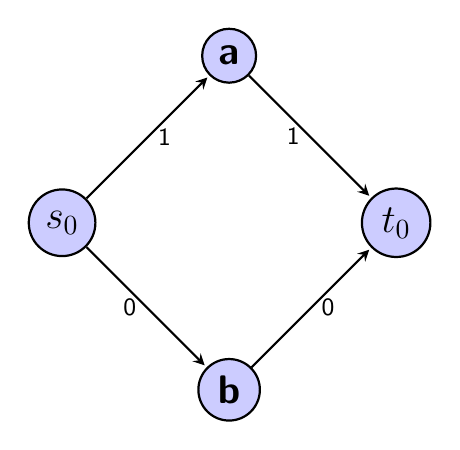
\begin{tikzpicture}[->,>=stealth,shorten >=1pt,auto,node distance=3cm,
 		thick,main node/.style={circle,fill=blue!20,draw,font=\sffamily\Large\bfseries}]

  		\node[main node] (B) {a};
  		\node[main node] (A) [below left of=B] {$s_0$};
  		\node[main node] (C) [below right of=A] {b};
  		\node[main node] (D) [below right of=B] {$t_0$};

  		\path[every node/.style={font=\sffamily\small}]
    		(B) edge node [left] {1} (D)
    		(A) edge node [right] {1} (B)
        		edge node [left]  {0} (C)
    		(C) edge node [right] {0} (D);
		\end{tikzpicture}
		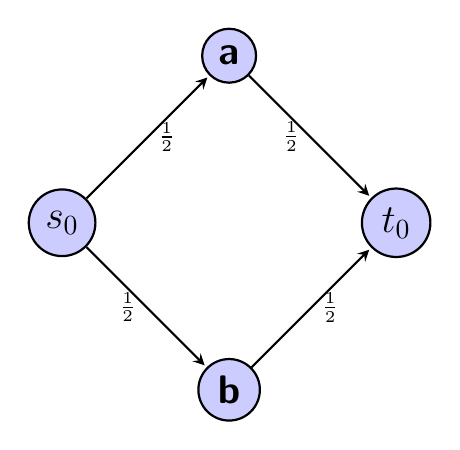
\begin{tikzpicture}[->,>=stealth,shorten >=1pt,auto,node distance=3cm,
 		thick,main node/.style={circle,fill=blue!20,draw,font=\sffamily\Large\bfseries}]

  		\node[main node] (B) {a};
  		\node[main node] (A) [below left of=B] {$s_0$};
  		\node[main node] (C) [below right of=A] {b};
  		\node[main node] (D) [below right of=B] {$t_0$};

  		\path[every node/.style={font=\sffamily\small}]
    		(B) edge node [left] {$\frac{1}{2}$} (D)
    		(A) edge node [right] {$\frac{1}{2}$} (B)
        		edge node [left]  {$\frac{1}{2}$} (C)
    		(C) edge node [right] {$\frac{1}{2}$} (D);
		\end{tikzpicture}\\
	\item This problem is very similar to proving the toll problem is the lower bound on the optimal solution to the path routing problem, so we will use similar conventions: $p_{ij}$ is a flow connecting $(s_i, t_i)$.  $c(e)$ is the congestion on edge $e$ under the routing.  The length of $p_{ij}$ is $d(p_{ij})$.  We proceed as in the integral problem, but the crux is that the lengths of the edges in a path do not necessarily add up to $1$: however, the sum of all the paths $p_{ij}$ connecting $(s_i, t_i)$ does.
		\begin{align*}
			\sum_{i}^{} \sum_{j}^{} d(p_{ij}) &= \sum_{i}^{} \sum_{j}^{} \sum_{e \in p_{ij}}^{} d(e) \\
			&= \sum_{e}^{} \sum_{i,j:e \in p_{ij}}^{} d(e) \\
			&= \sum_{e}^{} d(e) \sum_{i,j:e \in p_{ij}}^{} 1 \\
			&= \sum_{e}^{} d(e)c(e)
		\end{align*}
	\end{enumerate}
\item Equilibrium - pondered and completed but not written up.
\item Maximum weight matching vs. minimum weight vertex cover
	\begin{enumerate}
	\item Given $M$ a solution to the maximum weight matching problem and $p(\cdot)$ a solution to the minimum price vertex cover: $M=p(\cdot)$ iff the edges in the matching are tight and there is a perfect matching.  Both of these are satisfied, $\therefore M=p(\cdot)$.  When we increase the weight of an edge $(u,v)$ in our bipartite graph by $\delta$...
	\begin{algorithmic}
	\State $p(u) \gets p(u) + \delta$
	\If{$(u,v) \in M$}
		\Return
	\Else
		\State \textbf{find} $(u, v_1) \in M$ where $p(u) + p(v_1) > (u, v_1)$
		\State \# this must exist because we raised the price on $u$,
		\State \# so some edge in the matching,
		\State \# which does match $u$ because it is perfect,
		\State \# is no longer tight
		\State remove $(u, v_1)$ from $M$
		\State \textbf{continue} algorithm as usual, searching for an augmenting path
	\EndIf
	\end{algorithmic}
	\item If $m$ is the edges and $n$ is the vertices, then no.  Given that the last line says ``continue algorithm as usual'', we get the same runtime as the ``algorithm as usual'', which is to say $O(n^2 m)$ for the algorithm discussed in class.  Our piece for solving when we increase an edge weight by $\delta$ adds a complexity of $O(n/2)$ because we check all the edges leading to all the vertices in $V$ to determine which one is matched before dropping it from the matching, but as usual this term is ignored because the $O(n^2 m)$ term is much larger.
	\end{enumerate}
\end{enumerate}
\end{document}